\documentclass{standalone}
\usepackage{tikz}
\usetikzlibrary{patterns, positioning}
\usepackage[sfdefault]{ClearSans} %% option 'sfdefault' activates Clear Sans as the default text font
\usepackage[T1]{fontenc}

\begin{document}
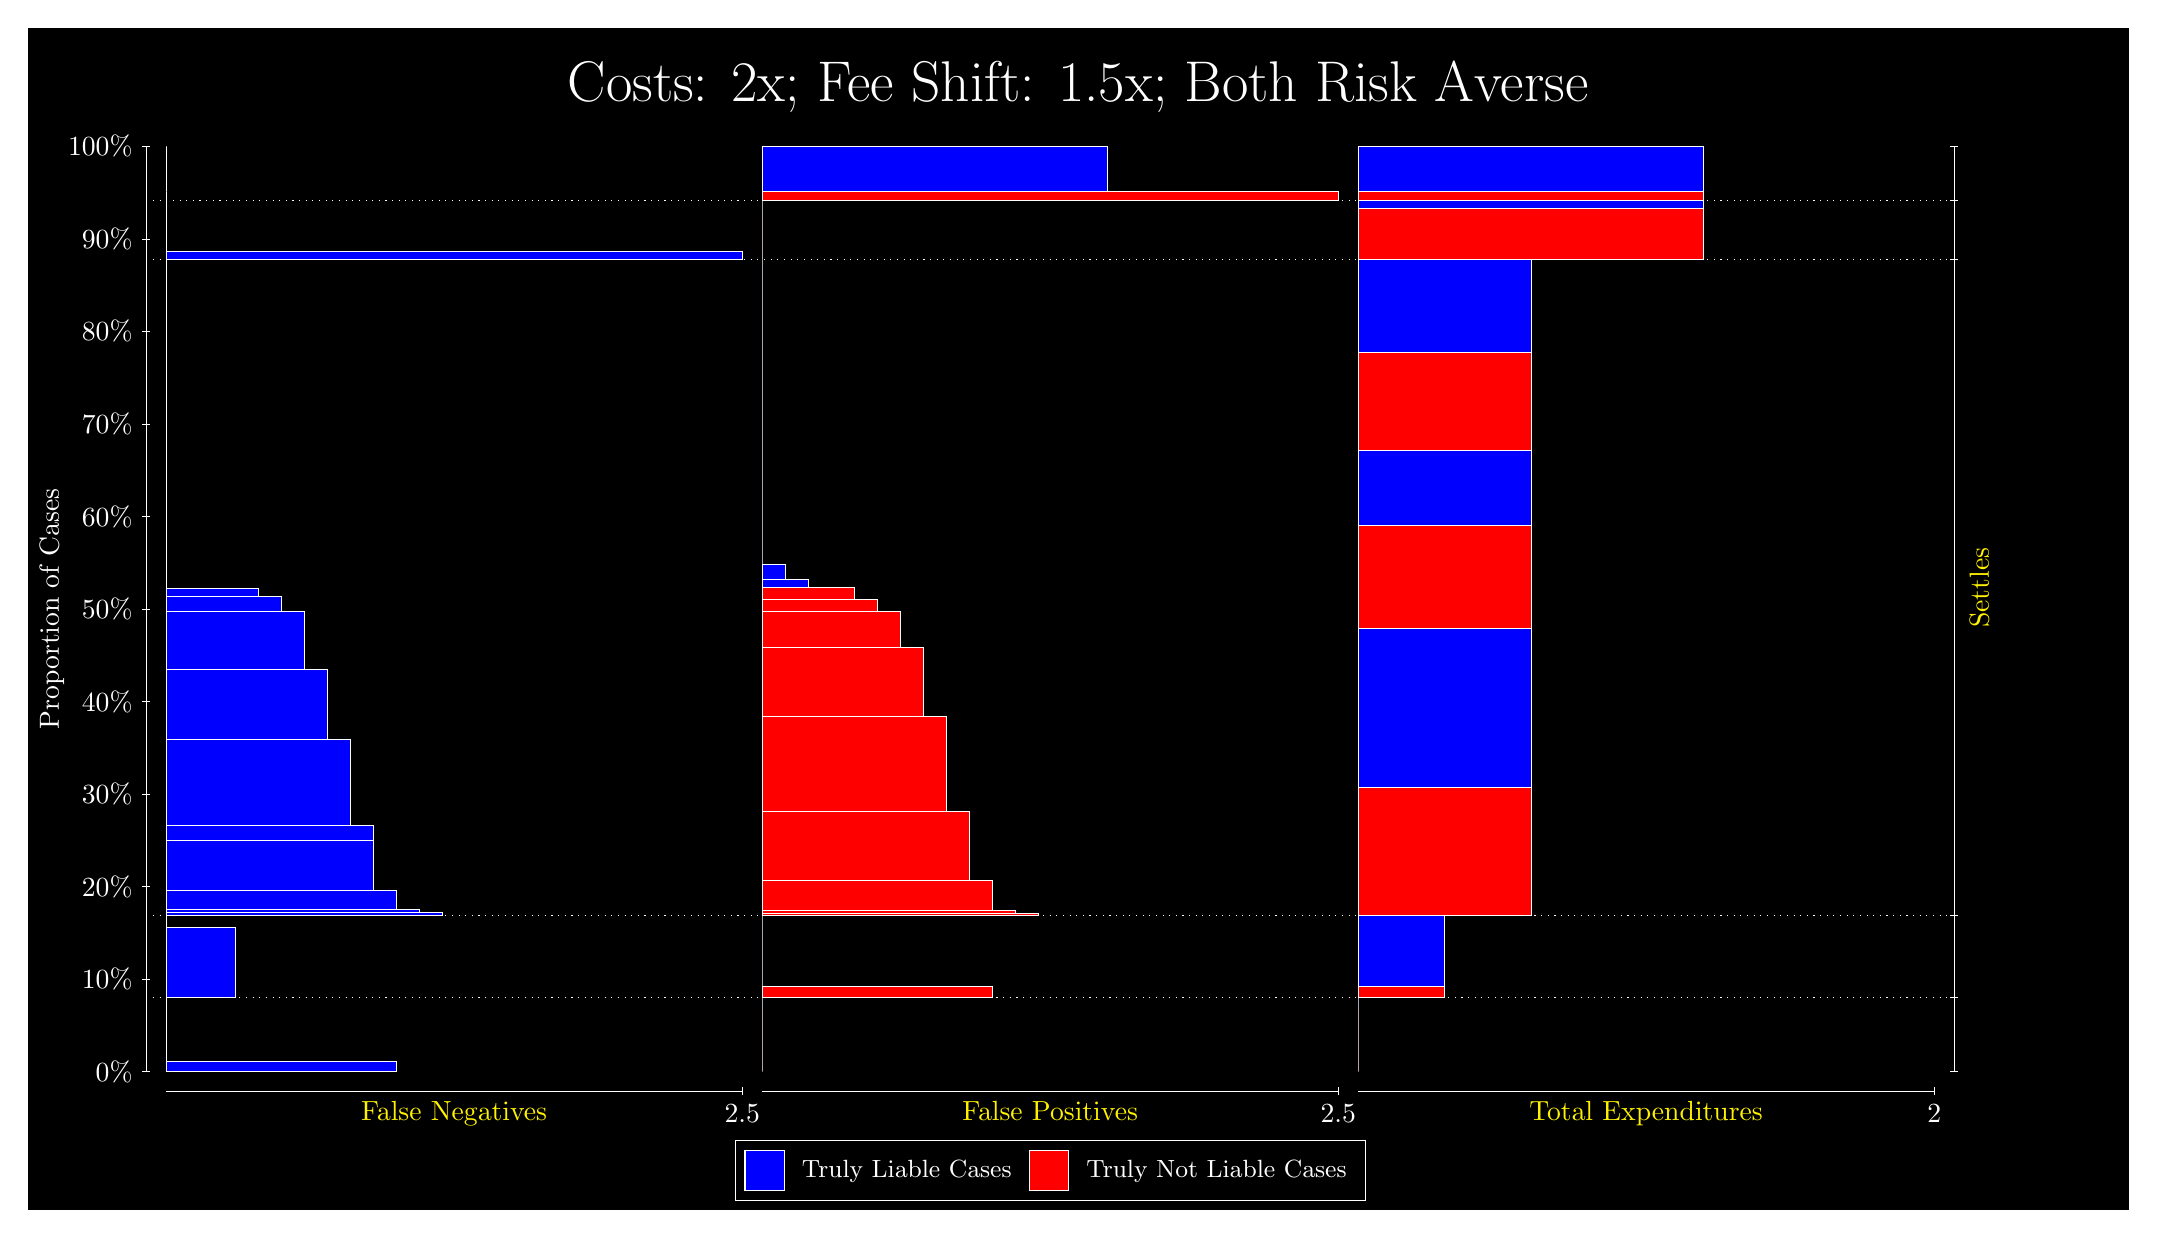
\begin{tikzpicture}
\draw[fill=black] (0,0) rectangle (26.667,15);
\draw[text=white] (0,13.5) rectangle (26.667,15) node[midway] {\huge Costs: 2x; Fee Shift: 1.5x; Both Risk Averse};
\draw[white, very thin] (1.5,1.75) -- (1.5,13.5);
\node[rotate=90, text=white, anchor=center] at (0.3, 7.625) {Proportion of Cases};
\draw[white, very thin] (1.45,1.75) -- (1.55,1.75);
\node[text=white, anchor=east] at (1.45, 1.75) {0\%};
\draw[white, very thin] (1.45,2.925) -- (1.55,2.925);
\node[text=white, anchor=east] at (1.45, 2.925) {10\%};
\draw[white, very thin] (1.45,4.1) -- (1.55,4.1);
\node[text=white, anchor=east] at (1.45, 4.1) {20\%};
\draw[white, very thin] (1.45,5.275) -- (1.55,5.275);
\node[text=white, anchor=east] at (1.45, 5.275) {30\%};
\draw[white, very thin] (1.45,6.45) -- (1.55,6.45);
\node[text=white, anchor=east] at (1.45, 6.45) {40\%};
\draw[white, very thin] (1.45,7.625) -- (1.55,7.625);
\node[text=white, anchor=east] at (1.45, 7.625) {50\%};
\draw[white, very thin] (1.45,8.8) -- (1.55,8.8);
\node[text=white, anchor=east] at (1.45, 8.8) {60\%};
\draw[white, very thin] (1.45,9.975) -- (1.55,9.975);
\node[text=white, anchor=east] at (1.45, 9.975) {70\%};
\draw[white, very thin] (1.45,11.15) -- (1.55,11.15);
\node[text=white, anchor=east] at (1.45, 11.15) {80\%};
\draw[white, very thin] (1.45,12.325) -- (1.55,12.325);
\node[text=white, anchor=east] at (1.45, 12.325) {90\%};
\draw[white, very thin] (1.45,13.5) -- (1.55,13.5);
\node[text=white, anchor=east] at (1.45, 13.5) {100\%};

\draw[white, very thin] (24.457,1.75) -- (24.457,13.5);
\draw[white, very thin] (24.407,1.75) -- (24.507,1.75);
\node[anchor=west] at (24.407, 1.75) {};
\draw[white, very thin] (24.407,2.6891) -- (24.507,2.6891);
\node[anchor=west] at (24.407, 2.6891) {};
\draw[white, very thin] (24.407,3.7304) -- (24.507,3.7304);
\node[anchor=west] at (24.407, 3.7304) {};
\draw[white, very thin] (24.407,12.06) -- (24.507,12.06);
\node[anchor=west] at (24.407, 12.06) {};
\draw[white, very thin] (24.407,12.816) -- (24.507,12.816);
\node[anchor=west] at (24.407, 12.816) {};
\draw[white, very thin] (24.407,13.5) -- (24.507,13.5);
\node[anchor=west] at (24.407, 13.5) {};

\draw[white, very thin, fill=blue] (1.75,1.75) rectangle (4.6775,1.8818);
\draw[white, very thin, fill=red] (1.75,1.8818) rectangle (1.75,2.6891);
\draw[white, very thin, fill=blue] (1.75,2.6891) rectangle (2.6283,3.5865);
\draw[white, very thin, fill=red] (1.75,3.5865) rectangle (1.75,3.7304);
\draw[white, very thin, fill=blue] (1.75,3.7304) rectangle (5.2631,3.7705);
\draw[white, very thin, fill=blue] (1.75,3.7705) rectangle (4.9703,3.8095);
\draw[white, very thin, fill=blue] (1.75,3.8095) rectangle (4.6775,4.0481);
\draw[white, very thin, fill=blue] (1.75,4.0481) rectangle (4.3848,4.6844);
\draw[white, very thin, fill=blue] (1.75,4.6844) rectangle (4.3848,4.8759);
\draw[white, very thin, fill=blue] (1.75,4.8759) rectangle (4.092,5.9724);
\draw[white, very thin, fill=blue] (1.75,5.9724) rectangle (3.7993,6.8544);
\draw[white, very thin, fill=blue] (1.75,6.8544) rectangle (3.5065,7.5987);
\draw[white, very thin, fill=blue] (1.75,7.5987) rectangle (3.2138,7.7865);
\draw[white, very thin, fill=blue] (1.75,7.7865) rectangle (2.921,7.892);
\draw[white, very thin, fill=red] (1.75,7.892) rectangle (1.75,12.06);
\draw[white, very thin, fill=blue] (1.75,12.06) rectangle (9.0689,12.169);
\draw[white, very thin, fill=red] (1.75,12.169) rectangle (1.75,12.816);
\draw[white, very thin, fill=red] (1.75,12.816) rectangle (1.75,12.925);
\draw[white, very thin, fill=blue] (1.75,12.925) rectangle (1.75,13.5);
\draw[white, very thin, fill=red] (9.3189,1.75) rectangle (9.3189,2.5573);
\draw[white, very thin, fill=blue] (9.3189,2.5573) rectangle (9.3189,2.6891);
\draw[white, very thin, fill=red] (9.3189,2.6891) rectangle (12.246,2.833);
\draw[white, very thin, fill=blue] (9.3189,2.833) rectangle (9.3189,3.7304);
\draw[white, very thin, fill=red] (9.3189,3.7304) rectangle (12.832,3.7612);
\draw[white, very thin, fill=red] (9.3189,3.7612) rectangle (12.539,3.8038);
\draw[white, very thin, fill=red] (9.3189,3.8038) rectangle (12.246,4.181);
\draw[white, very thin, fill=red] (9.3189,4.181) rectangle (11.954,5.0595);
\draw[white, very thin, fill=red] (9.3189,5.0595) rectangle (11.661,6.2662);
\draw[white, very thin, fill=red] (9.3189,6.2662) rectangle (11.368,7.1368);
\draw[white, very thin, fill=red] (9.3189,7.1368) rectangle (11.075,7.601);
\draw[white, very thin, fill=red] (9.3189,7.601) rectangle (10.783,7.7463);
\draw[white, very thin, fill=red] (9.3189,7.7463) rectangle (10.49,7.8986);
\draw[white, very thin, fill=blue] (9.3189,7.8986) rectangle (9.9044,8.004);
\draw[white, very thin, fill=blue] (9.3189,8.004) rectangle (9.6116,8.1918);
\draw[white, very thin, fill=blue] (9.3189,8.1918) rectangle (9.3189,12.06);
\draw[white, very thin, fill=red] (9.3189,12.06) rectangle (9.3189,12.707);
\draw[white, very thin, fill=blue] (9.3189,12.707) rectangle (9.3189,12.816);
\draw[white, very thin, fill=red] (9.3189,12.816) rectangle (16.638,12.925);
\draw[white, very thin, fill=blue] (9.3189,12.925) rectangle (13.71,13.5);
\draw[white, very thin, fill=red] (16.888,1.75) rectangle (16.888,2.5573);
\draw[white, very thin, fill=blue] (16.888,2.5573) rectangle (16.888,2.6891);
\draw[white, very thin, fill=red] (16.888,2.6891) rectangle (17.986,2.833);
\draw[white, very thin, fill=blue] (16.888,2.833) rectangle (17.986,3.7304);
\draw[white, very thin, fill=red] (16.888,3.7304) rectangle (19.083,5.3569);
\draw[white, very thin, fill=blue] (16.888,5.3569) rectangle (19.083,7.3854);
\draw[white, very thin, fill=red] (16.888,7.3854) rectangle (19.083,8.6887);
\draw[white, very thin, fill=blue] (16.888,8.6887) rectangle (19.083,9.6427);
\draw[white, very thin, fill=red] (16.888,9.6427) rectangle (19.083,10.881);
\draw[white, very thin, fill=blue] (16.888,10.881) rectangle (19.083,12.06);
\draw[white, very thin, fill=red] (16.888,12.06) rectangle (21.279,12.707);
\draw[white, very thin, fill=blue] (16.888,12.707) rectangle (21.279,12.816);
\draw[white, very thin, fill=red] (16.888,12.816) rectangle (21.279,12.925);
\draw[white, very thin, fill=blue] (16.888,12.925) rectangle (21.279,13.5);
\draw[white, dotted] (1.5,2.6891) -- (24.457,2.6891);
\draw[white, dotted] (1.5,3.7304) -- (24.457,3.7304);
\draw[white, dotted] (1.5,12.06) -- (24.457,12.06);
\draw[white, dotted] (1.5,12.816) -- (24.457,12.816);
\draw[white, very thin] (1.75,1.5) -- (9.0689,1.5);
\node[text=yellow, anchor=north] at (5.4094, 1.5) {False Negatives};
\draw[white, very thin] (9.0689,1.45) -- (9.0689,1.55);
\node[text=white, anchor=north] at (9.0689, 1.45) {2.5};

\draw[white, very thin] (9.3189,1.5) -- (16.638,1.5);
\node[text=yellow, anchor=north] at (12.978, 1.5) {False Positives};
\draw[white, very thin] (16.638,1.45) -- (16.638,1.55);
\node[text=white, anchor=north] at (16.638, 1.45) {2.5};

\draw[white, very thin] (16.888,1.5) -- (24.207,1.5);
\node[text=yellow, anchor=north] at (20.547, 1.5) {Total Expenditures};
\draw[white, very thin] (24.207,1.45) -- (24.207,1.55);
\node[text=white, anchor=north] at (24.207, 1.45) {2};



\node[text=yellow, centered, rotate=90] at (24.777, 7.8953) {Settles};



\draw (12.978300999999998,1.5) node[draw=none] (baseCoordinate) {};
\begin{scope}[align=center]
        \matrix[scale=0.5, draw=white, below=0.5cm of baseCoordinate, nodes={draw}, column sep=0.1cm]{
            \node[rectangle, draw, minimum width=0.5cm, minimum height=0.5cm, fill=blue] {}; &
            \node[draw=none, font=\small, text=white] (B) {Truly Liable Cases}; &
            \node[rectangle, draw, minimum width=0.5cm, minimum height=0.5cm, fill=red] {}; &
            \node[draw=none, font=\small, text=white] (B) {Truly Not Liable Cases}; \\
            };
\end{scope}

\end{tikzpicture}
\end{document}